\documentclass{article}\usepackage[]{graphicx}\usepackage[]{xcolor}
% maxwidth is the original width if it is less than linewidth
% otherwise use linewidth (to make sure the graphics do not exceed the margin)
\makeatletter
\def\maxwidth{ %
  \ifdim\Gin@nat@width>\linewidth
    \linewidth
  \else
    \Gin@nat@width
  \fi
}
\makeatother

\definecolor{fgcolor}{rgb}{0.345, 0.345, 0.345}
\newcommand{\hlnum}[1]{\textcolor[rgb]{0.686,0.059,0.569}{#1}}%
\newcommand{\hlsng}[1]{\textcolor[rgb]{0.192,0.494,0.8}{#1}}%
\newcommand{\hlcom}[1]{\textcolor[rgb]{0.678,0.584,0.686}{\textit{#1}}}%
\newcommand{\hlopt}[1]{\textcolor[rgb]{0,0,0}{#1}}%
\newcommand{\hldef}[1]{\textcolor[rgb]{0.345,0.345,0.345}{#1}}%
\newcommand{\hlkwa}[1]{\textcolor[rgb]{0.161,0.373,0.58}{\textbf{#1}}}%
\newcommand{\hlkwb}[1]{\textcolor[rgb]{0.69,0.353,0.396}{#1}}%
\newcommand{\hlkwc}[1]{\textcolor[rgb]{0.333,0.667,0.333}{#1}}%
\newcommand{\hlkwd}[1]{\textcolor[rgb]{0.737,0.353,0.396}{\textbf{#1}}}%
\let\hlipl\hlkwb

\usepackage{framed}
\makeatletter
\newenvironment{kframe}{%
 \def\at@end@of@kframe{}%
 \ifinner\ifhmode%
  \def\at@end@of@kframe{\end{minipage}}%
  \begin{minipage}{\columnwidth}%
 \fi\fi%
 \def\FrameCommand##1{\hskip\@totalleftmargin \hskip-\fboxsep
 \colorbox{shadecolor}{##1}\hskip-\fboxsep
     % There is no \\@totalrightmargin, so:
     \hskip-\linewidth \hskip-\@totalleftmargin \hskip\columnwidth}%
 \MakeFramed {\advance\hsize-\width
   \@totalleftmargin\z@ \linewidth\hsize
   \@setminipage}}%
 {\par\unskip\endMakeFramed%
 \at@end@of@kframe}
\makeatother

\definecolor{shadecolor}{rgb}{.97, .97, .97}
\definecolor{messagecolor}{rgb}{0, 0, 0}
\definecolor{warningcolor}{rgb}{1, 0, 1}
\definecolor{errorcolor}{rgb}{1, 0, 0}
\newenvironment{knitrout}{}{} % an empty environment to be redefined in TeX

\usepackage{alltt}
\usepackage[margin=1.0in]{geometry} % To set margins
\usepackage{amsmath}  % This allows me to use the align functionality.
% If you find yourself trying to replicate
% something you found online, ensure you're
% loading the necessary packages!
\usepackage{amsfonts} % Math font
\usepackage{fancyvrb}
\usepackage{hyperref} % For including hyperlinks
\usepackage[shortlabels]{enumitem}% For enumerated lists with labels specified
% We had to run tlmgr_install("enumitem") in R
\usepackage{float}    % For telling R where to put a table/figure
\usepackage{natbib}        %For the bibliography
\bibliographystyle{apalike}%For the bibliography
\IfFileExists{upquote.sty}{\usepackage{upquote}}{}
\begin{document}
\noindent\textbf{Homework 4: ANOVA and Kruskal-Wallis}\\
\noindent\makebox[\linewidth]{\rule{\textwidth}{0.4pt}}
\noindent\underline{Submission Notes:} Please write your answers to each 
question under that question (not altogether at the end). It will be easier for 
me to give full credit if your answer is commented well, including comments 
about where you are completing each sub-part of the question. For an example,
see Homework 1.\\
\noindent\makebox[\linewidth]{\rule{\textwidth}{0.4pt}}


\begin{enumerate}
%%%%%%%%%%%%%%%%%%%%%%%%%%%%%%%%%%%%%%%%%%%%%%%%%%%%%%%%%%%%%%%%%%%%%%%%%%%%%%%%
%%%%%%%%%%%%%%%%%%%%%%%%%%%%%%%%%%%%%%%%%%%%%%%%%%%%%%%%%%%%%%%%%%%%%%%%%%%%%%%%
% Question 1
%%%%%%%%%%%%%%%%%%%%%%%%%%%%%%%%%%%%%%%%%%%%%%%%%%%%%%%%%%%%%%%%%%%%%%%%%%%%%%%%
%%%%%%%%%%%%%%%%%%%%%%%%%%%%%%%%%%%%%%%%%%%%%%%%%%%%%%%%%%%%%%%%%%%%%%%%%%%%%%%%
\item \textbf{What are we doing?} On Homework 3 and the exam, it is clear that
the process of statistical inference is still a little murky. I think the 
challenge is that the process changes with each test, so it gets a bit hard
to see the big picture. Let's try to see if we can peel back some layers here
by exploring how important mathematical statisticians are.\\

First, we have discussed the ANOVA test. When all $k$ population means are 
equal, all $k$ population distributions are Gaussian, all $k$ samples are
of the same size, and all $k$ population variances are equal, mathematical 
statisticians can show that
\[F = \frac{\frac{1}{k-1} \sum_{i=1}^k \left(\bar{X}_{i\cdot}-\bar{X}_{\cdot\cdot}\right)^2}{\sum_{i=1}^k\left(\frac{n_i-1}{N-k}\right)S_i^2} \sim F(N-k, k-1).\]
Note that you can compute this statistic for $k=3$ using the following code:
\begin{knitrout}\scriptsize
\definecolor{shadecolor}{rgb}{0.969, 0.969, 0.969}\color{fgcolor}\begin{kframe}
\begin{alltt}
\hldef{xbar1} \hlkwb{<-} \hlkwd{mean}\hldef{(x1)}
\hldef{xbar2} \hlkwb{<-} \hlkwd{mean}\hldef{(x2)}
\hldef{xbar3} \hlkwb{<-} \hlkwd{mean}\hldef{(x3)}
\hldef{X} \hlkwb{<-} \hlkwd{c}\hldef{(x1, x2, x3)}
\hldef{xbar} \hlkwb{<-} \hlkwd{mean}\hldef{(X)}
\hlcom{# SSBetween}
\hldef{SSB} \hlkwb{<-} \hldef{n1}\hlopt{*}\hldef{(xbar1}\hlopt{-}\hldef{xbar)}\hlopt{^}\hlnum{2} \hlopt{+} \hldef{n2}\hlopt{*}\hldef{(xbar2}\hlopt{-}\hldef{xbar)}\hlopt{^}\hlnum{2} \hlopt{+} \hldef{n3}\hlopt{*}\hldef{(xbar3}\hlopt{-}\hldef{xbar)}\hlopt{^}\hlnum{2}
\hlcom{# SSWithin}
\hldef{SSW} \hlkwb{<-} \hldef{(n1}\hlopt{-}\hlnum{1}\hldef{)}\hlopt{*}\hlkwd{var}\hldef{(x1)} \hlopt{+} \hldef{(n2}\hlopt{-}\hlnum{1}\hldef{)}\hlopt{*}\hlkwd{var}\hldef{(x2)} \hlopt{+} \hldef{(n3}\hlopt{-}\hlnum{1}\hldef{)}\hlopt{*}\hlkwd{var}\hldef{(x3)}
\hlcom{# F-statistic}
\hldef{F.stat[i]} \hlkwb{<-} \hldef{(SSB}\hlopt{/}\hldef{(k}\hlopt{-}\hlnum{1}\hldef{))}\hlopt{/}\hldef{(SSW}\hlopt{/}\hldef{(N}\hlopt{-}\hldef{k))}
\end{alltt}
\end{kframe}
\end{knitrout}
A nonparametric alternative to the ANOVA test is the Kruskal-Wallis test. When 
all $k$ population means are equal and all $k$ population distributions are the
the same shape, mathematical statisticians can show that for large $n$
\begin{align*}
H &= \frac{\textrm{Sum of Squared Deviations of the Sample Rank Sums}}{\textrm{Sum of Squares for Ranks }1, 2, ..., N}\\
&= \frac{\sum_{i=1}^k n_i(\bar{R}_{i\cdot} - \bar{R}_{\cdot\cdot})^2}{\frac{N(N+1)}{12}}\\
&= \left(\frac{12}{N(N+1)}\right) \sum_{i=1}^k \frac{\left(\sum_{j=1}^{n_i} r_{ij}\right)^2}{n_i}
- 3(N+1) \tag{Simplified Computing Formula}\\
& \sim \mathcal{A}\chi^2(v=k-1)
\end{align*}
where $r_{ij}$ is the rank of the $j$th observation in sample $i$, and the 
normalizing constant enables us to use the $\chi^2(v=k-1)$ distribution.\\

When there are no ties, the $H$ statistic is equivalent to the $F$ statistic 
computed on the ranks. The top is the between estimator and the bottom is
the within, noting the data will always be 1, 2, ..., N when there are no
ties.\\

When there are ties, we adjust the $H$ statistic by dividing by
\[t_{adj} = 1 - \frac{\sum_{r=1}^{\max(r)} o_r^3-o_r}{N^3-N}\]
where $o_r$ is the number of times rank $r$ occurs.\\

Note that you can compute this statistic for $k=3$ using the following code:
\begin{knitrout}\scriptsize
\definecolor{shadecolor}{rgb}{0.969, 0.969, 0.969}\color{fgcolor}\begin{kframe}
\begin{alltt}
\hldef{X} \hlkwb{<-} \hlkwd{c}\hldef{(x1, x2, x3)}
\hldef{ranks} \hlkwb{<-} \hlkwd{rank}\hldef{(X)}
\hldef{r1} \hlkwb{<-} \hldef{ranks[}\hlnum{1}\hlopt{:}\hlkwd{length}\hldef{(x1)]}
\hldef{r2} \hlkwb{<-} \hldef{ranks[(n1}\hlopt{+}\hlnum{1}\hldef{)}\hlopt{:}\hldef{(n1}\hlopt{+}\hldef{n2)]}
\hldef{r3} \hlkwb{<-} \hldef{ranks[(n1}\hlopt{+}\hldef{n2}\hlopt{+}\hlnum{1}\hldef{)}\hlopt{:}\hldef{N]}
\hlcom{# Rank Sums}
\hldef{rank.sums} \hlkwb{<-} \hlnum{12}\hlopt{/}\hldef{(N}\hlopt{*}\hldef{(N}\hlopt{+}\hlnum{1}\hldef{))} \hlopt{*} \hldef{(}\hlkwd{sum}\hldef{(r1)}\hlopt{^}\hlnum{2}\hlopt{/}\hldef{n1} \hlopt{+} \hlkwd{sum}\hldef{(r2)}\hlopt{^}\hlnum{2}\hlopt{/}\hldef{n2} \hlopt{+} \hlkwd{sum}\hldef{(r3)}\hlopt{^}\hlnum{2}\hlopt{/}\hldef{n3)}
\hlcom{# Ties? (Note: when there are no ties, this adjustment is 1)}
\hldef{ties.adj} \hlkwb{<-} \hlkwd{tibble}\hldef{(}\hlkwc{r}\hldef{=ranks) |>} \hlcom{# create a tibble}
  \hlkwd{group_by}\hldef{(r) |>}               \hlcom{# group by the ranks}
  \hlkwd{summarize}\hldef{(}\hlkwc{n}\hldef{=}\hlkwd{n}\hldef{())|>}           \hlcom{# count the number of unique ranks}
  \hlkwd{summarize}\hldef{(}\hlkwc{ties.adj} \hldef{=} \hlnum{1}\hlopt{-}\hlkwd{sum}\hldef{(n}\hlopt{^}\hlnum{3}\hlopt{-}\hldef{n)}\hlopt{/}\hldef{(N}\hlopt{^}\hlnum{3}\hlopt{-}\hldef{N))|>} \hlcom{# compute adjustment}
  \hlkwd{pull}\hldef{()} \hlcom{# convert from tibble to numeric}
\hlcom{# H-statistic}
\hldef{H.stat[i]} \hlkwb{<-} \hldef{(rank.sums} \hlopt{-} \hlnum{3}\hlopt{*}\hldef{(N}\hlopt{+}\hlnum{1}\hldef{))}\hlopt{/}\hldef{ties.adj}
\end{alltt}
\end{kframe}
\end{knitrout}
For 1000 simulations, simulate \texttt{x1}, \texttt{x2}, \texttt{x3} from the 
Gaussian distribution with 
\begin{itemize}
\item $n_1=58$, $n_2=72$, and $n_3=63$
\item $\mu_1=\mu_2=\mu_3=2$
\item $\sigma_1=\sigma_2=\sigma_3=5$,
\end{itemize}
and compute the $F$ and $H$ statistics.

\begin{knitrout}\scriptsize
\definecolor{shadecolor}{rgb}{0.969, 0.969, 0.969}\color{fgcolor}\begin{kframe}
\begin{alltt}
\hlkwd{library}\hldef{(tidyverse)}

\hlkwd{set.seed}\hldef{(}\hlnum{1313}\hldef{)}

\hldef{n1} \hlkwb{=} \hlnum{58}
\hldef{n2} \hlkwb{=} \hlnum{72}
\hldef{n3} \hlkwb{=} \hlnum{63}
\hldef{N} \hlkwb{=} \hldef{n1} \hlopt{+} \hldef{n2} \hlopt{+} \hldef{n3}
\hldef{mu} \hlkwb{=} \hlnum{2}
\hldef{sigma} \hlkwb{=} \hlnum{5}
\hldef{k} \hlkwb{=} \hlnum{3}
\hldef{F.stat} \hlkwb{<-} \hlkwd{rep}\hldef{(}\hlnum{NA}\hldef{,} \hlnum{1000}\hldef{)}
\hldef{H.stat} \hlkwb{<-} \hlkwd{rep}\hldef{(}\hlnum{NA}\hldef{,} \hlnum{1000}\hldef{)}

\hlkwa{for} \hldef{(i} \hlkwa{in} \hlnum{1}\hlopt{:}\hlnum{1000}\hldef{)\{}

  \hldef{x1} \hlkwb{=} \hlkwd{rnorm}\hldef{(}\hlkwc{n} \hldef{= n1,} \hlkwc{mean} \hldef{= mu,} \hlkwc{sd} \hldef{= sigma)}
  \hldef{x2} \hlkwb{=} \hlkwd{rnorm}\hldef{(}\hlkwc{n} \hldef{= n2,} \hlkwc{mean} \hldef{= mu,} \hlkwc{sd} \hldef{= sigma)}
  \hldef{x3} \hlkwb{=} \hlkwd{rnorm}\hldef{(}\hlkwc{n} \hldef{= n3,} \hlkwc{mean} \hldef{= mu,} \hlkwc{sd} \hldef{= sigma)}

  \hlcom{# ANOVA F stat}
  \hldef{xbar1} \hlkwb{<-} \hlkwd{mean}\hldef{(x1)}
  \hldef{xbar2} \hlkwb{<-} \hlkwd{mean}\hldef{(x2)}
  \hldef{xbar3} \hlkwb{<-} \hlkwd{mean}\hldef{(x3)}
  \hldef{X} \hlkwb{<-} \hlkwd{c}\hldef{(x1, x2, x3)}
  \hldef{xbar} \hlkwb{<-} \hlkwd{mean}\hldef{(X)}
  \hlcom{# SSBetween}
  \hldef{SSB} \hlkwb{<-} \hldef{n1}\hlopt{*}\hldef{(xbar1}\hlopt{-}\hldef{xbar)}\hlopt{^}\hlnum{2} \hlopt{+} \hldef{n2}\hlopt{*}\hldef{(xbar2}\hlopt{-}\hldef{xbar)}\hlopt{^}\hlnum{2} \hlopt{+} \hldef{n3}\hlopt{*}\hldef{(xbar3}\hlopt{-}\hldef{xbar)}\hlopt{^}\hlnum{2}
  \hlcom{# SSWithin}
  \hldef{SSW} \hlkwb{<-} \hldef{(n1}\hlopt{-}\hlnum{1}\hldef{)}\hlopt{*}\hlkwd{var}\hldef{(x1)} \hlopt{+} \hldef{(n2}\hlopt{-}\hlnum{1}\hldef{)}\hlopt{*}\hlkwd{var}\hldef{(x2)} \hlopt{+} \hldef{(n3}\hlopt{-}\hlnum{1}\hldef{)}\hlopt{*}\hlkwd{var}\hldef{(x3)}
  \hlcom{# F-statistic}
  \hldef{F.stat[i]} \hlkwb{<-} \hldef{(SSB}\hlopt{/}\hldef{(k}\hlopt{-}\hlnum{1}\hldef{))}\hlopt{/}\hldef{(SSW}\hlopt{/}\hldef{(N}\hlopt{-}\hldef{k))}

  \hlcom{# KW H stat}
  \hldef{X} \hlkwb{<-} \hlkwd{c}\hldef{(x1, x2, x3)}
  \hldef{ranks} \hlkwb{<-} \hlkwd{rank}\hldef{(X)}
  \hldef{r1} \hlkwb{<-} \hldef{ranks[}\hlnum{1}\hlopt{:}\hlkwd{length}\hldef{(x1)]}
  \hldef{r2} \hlkwb{<-} \hldef{ranks[(n1}\hlopt{+}\hlnum{1}\hldef{)}\hlopt{:}\hldef{(n1}\hlopt{+}\hldef{n2)]}
  \hldef{r3} \hlkwb{<-} \hldef{ranks[(n1}\hlopt{+}\hldef{n2}\hlopt{+}\hlnum{1}\hldef{)}\hlopt{:}\hldef{N]}
  \hlcom{# Rank Sums}
  \hldef{rank.sums} \hlkwb{<-} \hlnum{12}\hlopt{/}\hldef{(N}\hlopt{*}\hldef{(N}\hlopt{+}\hlnum{1}\hldef{))} \hlopt{*} \hldef{(}\hlkwd{sum}\hldef{(r1)}\hlopt{^}\hlnum{2}\hlopt{/}\hldef{n1} \hlopt{+} \hlkwd{sum}\hldef{(r2)}\hlopt{^}\hlnum{2}\hlopt{/}\hldef{n2} \hlopt{+} \hlkwd{sum}\hldef{(r3)}\hlopt{^}\hlnum{2}\hlopt{/}\hldef{n3)}
  \hlcom{# Ties? (Note: when there are no ties, this adjustment is 1)}
  \hldef{ties.adj} \hlkwb{<-} \hlkwd{tibble}\hldef{(}\hlkwc{r}\hldef{=ranks) |>} \hlcom{# create a tibble}
    \hlkwd{group_by}\hldef{(r) |>}               \hlcom{# group by the ranks}
    \hlkwd{summarize}\hldef{(}\hlkwc{n}\hldef{=}\hlkwd{n}\hldef{())|>}           \hlcom{# count the number of unique ranks}
    \hlkwd{summarize}\hldef{(}\hlkwc{ties.adj} \hldef{=} \hlnum{1}\hlopt{-}\hlkwd{sum}\hldef{(n}\hlopt{^}\hlnum{3}\hlopt{-}\hldef{n)}\hlopt{/}\hldef{(N}\hlopt{^}\hlnum{3}\hlopt{-}\hldef{N))|>} \hlcom{# compute adjustment}
    \hlkwd{pull}\hldef{()} \hlcom{# convert from tibble to numeric}
  \hlcom{# H-statistic}
  \hldef{H.stat[i]} \hlkwb{<-} \hldef{(rank.sums} \hlopt{-} \hlnum{3}\hlopt{*}\hldef{(N}\hlopt{+}\hlnum{1}\hldef{))}\hlopt{/}\hldef{ties.adj}

\hldef{\}}
\end{alltt}
\end{kframe}
\end{knitrout}

\begin{enumerate}
\item Plot a histogram of the $F$ statistics and overlay the sampling 
distribution described by mathematical statisticians. Include a vertical
line denoting the $F$ statistic where the rejection region starts. What
do you note about the histogram and the corresponding $F$ distribution?

\begin{figure}[H]

\centering

\begin{knitrout}\scriptsize
\definecolor{shadecolor}{rgb}{0.969, 0.969, 0.969}\color{fgcolor}\begin{kframe}
\begin{alltt}
\hldef{F_dist} \hlkwb{<-} \hlkwd{tibble}\hldef{(}\hlkwc{F.stat} \hldef{=} \hlkwd{seq}\hldef{(}\hlkwc{from} \hldef{=} \hlnum{0}\hldef{,}
                              \hlkwc{to} \hldef{=} \hlnum{10}\hldef{,}
                              \hlkwc{length.out} \hldef{=} \hlnum{10000}\hldef{)) |>}
  \hlkwd{mutate}\hldef{(}\hlkwc{density} \hldef{=} \hlkwd{df}\hldef{(F.stat,} \hlkwc{df1} \hldef{= k}\hlopt{-}\hlnum{1}\hldef{,} \hlkwc{df2} \hldef{= N}\hlopt{-}\hldef{k))}

\hldef{rejection_point_F} \hlkwb{<-} \hlkwd{qf}\hldef{(}\hlkwc{p} \hldef{=} \hlnum{0.05}\hldef{,} \hlkwc{df1} \hldef{= k}\hlopt{-}\hlnum{1}\hldef{,} \hlkwc{df2} \hldef{= N}\hlopt{-}\hldef{k,} \hlkwc{lower.tail} \hldef{= F)}


\hlkwd{ggplot}\hldef{()} \hlopt{+}
  \hlkwd{geom_histogram}\hldef{(}\hlkwc{data} \hldef{=} \hlkwd{tibble}\hldef{(}\hlkwc{x} \hldef{= F.stat),} \hlkwd{aes}\hldef{(}\hlkwc{x} \hldef{= x,} \hlkwc{y} \hldef{=} \hlkwd{after_stat}\hldef{(density)),} \hlkwc{bins} \hldef{=} \hlnum{40}\hldef{)} \hlopt{+}
  \hlkwd{geom_line}\hldef{(}\hlkwc{data} \hldef{= F_dist,} \hlkwd{aes}\hldef{(}\hlkwc{x} \hldef{= F.stat,} \hlkwc{y} \hldef{= density))} \hlopt{+}
  \hlkwd{theme_bw}\hldef{()} \hlopt{+}
  \hlkwd{geom_hline}\hldef{(}\hlkwc{yintercept} \hldef{=} \hlnum{0}\hldef{)} \hlopt{+}
  \hlkwd{xlab}\hldef{(}\hlsng{"F"}\hldef{)} \hlopt{+}
  \hlkwd{ylab}\hldef{(}\hlsng{"Density"}\hldef{)} \hlopt{+}
  \hlkwd{geom_vline}\hldef{(}\hlkwc{xintercept} \hldef{= rejection_point_F,} \hlkwc{color} \hldef{=} \hlsng{"red"}\hldef{)}
\end{alltt}
\end{kframe}

\includegraphics[width=\maxwidth]{figure/unnamed-chunk-5-1} 
\end{knitrout}
\caption{Histogram of F values and the F Distribution}\label{F.hist}
\end{figure}


\textcolor{red}{The histogram and the F distribution match eachother almost identically, except fot the values very close to zero.}


\item Plot a histogram of the $H$ statistics and overlay the sampling 
distribution described by mathematical statisticians. Include a vertical
line denoting the chi-squared statistic where the rejection region starts.
What do you note about the histogram and the corresponding $\chi^2$ 
distribution?

\begin{figure}[H]

\centering

\begin{knitrout}\scriptsize
\definecolor{shadecolor}{rgb}{0.969, 0.969, 0.969}\color{fgcolor}\begin{kframe}
\begin{alltt}
\hldef{H_dist} \hlkwb{<-} \hlkwd{tibble}\hldef{(}\hlkwc{H.stat} \hldef{=} \hlkwd{seq}\hldef{(}\hlkwc{from} \hldef{=} \hlnum{0}\hldef{,}
                              \hlkwc{to} \hldef{=} \hlnum{12}\hldef{,}
                              \hlkwc{length.out} \hldef{=} \hlnum{10000}\hldef{)) |>}
  \hlkwd{mutate}\hldef{(}\hlkwc{density} \hldef{=} \hlkwd{dchisq}\hldef{(H.stat,} \hlkwc{df} \hldef{= k}\hlopt{-}\hlnum{1}\hldef{))}

\hldef{rejection_point_H} \hlkwb{<-} \hlkwd{qchisq}\hldef{(}\hlkwc{p} \hldef{=} \hlnum{0.05}\hldef{,} \hlkwc{df} \hldef{= k}\hlopt{-}\hlnum{1}\hldef{,} \hlkwc{lower.tail} \hldef{= F)}


\hlkwd{ggplot}\hldef{()} \hlopt{+}
  \hlkwd{geom_histogram}\hldef{(}\hlkwc{data} \hldef{=} \hlkwd{tibble}\hldef{(}\hlkwc{x} \hldef{= H.stat),} \hlkwd{aes}\hldef{(}\hlkwc{x} \hldef{= x,} \hlkwc{y} \hldef{=} \hlkwd{after_stat}\hldef{(density)),} \hlkwc{bins} \hldef{=} \hlnum{40}\hldef{)} \hlopt{+}
  \hlkwd{geom_line}\hldef{(}\hlkwc{data} \hldef{= H_dist,} \hlkwd{aes}\hldef{(}\hlkwc{x} \hldef{= H.stat,} \hlkwc{y} \hldef{= density))} \hlopt{+}
  \hlkwd{theme_bw}\hldef{()} \hlopt{+}
  \hlkwd{geom_hline}\hldef{(}\hlkwc{yintercept} \hldef{=} \hlnum{0}\hldef{)} \hlopt{+}
  \hlkwd{xlab}\hldef{(}\hlkwd{bquote}\hldef{(chi}\hlopt{^}\hlnum{2}\hldef{))} \hlopt{+}
  \hlkwd{ylab}\hldef{(}\hlsng{"Density"}\hldef{)} \hlopt{+}
  \hlkwd{geom_vline}\hldef{(}\hlkwc{xintercept} \hldef{= rejection_point_H,} \hlkwc{color} \hldef{=} \hlsng{"red"}\hldef{)}
\end{alltt}
\end{kframe}

\includegraphics[width=\maxwidth]{figure/unnamed-chunk-6-1} 
\end{knitrout}
\caption{Histogram of H values and the $\chi^2$ Distribution}\label{chi2.hist}
\end{figure}

\textcolor{red}{The H values also closely follow the $\chi^2$ distribution well.}

\item What proportion of the time did your simulation result in a statistic
in the rejection region for both tests?

\begin{knitrout}\scriptsize
\definecolor{shadecolor}{rgb}{0.969, 0.969, 0.969}\color{fgcolor}\begin{kframe}
\begin{alltt}
\hldef{(type1_error_F} \hlkwb{<-} \hlkwd{mean}\hldef{(F.stat} \hlopt{>=} \hldef{rejection_point_F))}
\end{alltt}
\begin{verbatim}
## [1] 0.048
\end{verbatim}
\begin{alltt}
\hldef{(type1_error_H} \hlkwb{<-} \hlkwd{mean}\hldef{(H.stat} \hlopt{>=} \hldef{rejection_point_H))}
\end{alltt}
\begin{verbatim}
## [1] 0.046
\end{verbatim}
\end{kframe}
\end{knitrout}


\item Now, let's assume our data are a bit misbehaved. That is, redo
(a)-(c) but now generate the data from a Laplace distribution with
\texttt{location} equal to $\mu_i$ and the \texttt{scale}=$\sigma_i/\sqrt{2}$.
What do you notice?\\
\textbf{Note:} You can find \texttt{rlaplace()} in the \texttt{VGAM}
package for \texttt{R} \cite{VGAM}.

\begin{knitrout}\scriptsize
\definecolor{shadecolor}{rgb}{0.969, 0.969, 0.969}\color{fgcolor}\begin{kframe}
\begin{alltt}
\hlkwd{library}\hldef{(VGAM)}

\hldef{F.stat_lap} \hlkwb{<-} \hlkwd{rep}\hldef{(}\hlnum{NA}\hldef{,} \hlnum{1000}\hldef{)}
\hldef{H.stat_lap} \hlkwb{<-} \hlkwd{rep}\hldef{(}\hlnum{NA}\hldef{,} \hlnum{1000}\hldef{)}

\hlkwa{for} \hldef{(i} \hlkwa{in} \hlnum{1}\hlopt{:}\hlnum{1000}\hldef{)\{}

\hldef{x1_lap} \hlkwb{<-} \hlkwd{rlaplace}\hldef{(}\hlkwc{n} \hldef{= n1,}
                   \hlkwc{location} \hldef{= mu,}
                   \hlkwc{scale} \hldef{= sigma}\hlopt{/}\hlkwd{sqrt}\hldef{(}\hlnum{2}\hldef{))}
\hldef{x2_lap} \hlkwb{<-} \hlkwd{rlaplace}\hldef{(}\hlkwc{n} \hldef{= n2,}
                   \hlkwc{location} \hldef{= mu,}
                   \hlkwc{scale} \hldef{= sigma}\hlopt{/}\hlkwd{sqrt}\hldef{(}\hlnum{2}\hldef{))}
\hldef{x3_lap} \hlkwb{<-} \hlkwd{rlaplace}\hldef{(}\hlkwc{n} \hldef{= n3,}
                   \hlkwc{location} \hldef{= mu,}
                   \hlkwc{scale} \hldef{= sigma}\hlopt{/}\hlkwd{sqrt}\hldef{(}\hlnum{2}\hldef{))}

  \hlcom{# ANOVA F stat}
  \hldef{xbar1_lap} \hlkwb{<-} \hlkwd{mean}\hldef{(x1_lap)}
  \hldef{xbar2_lap} \hlkwb{<-} \hlkwd{mean}\hldef{(x2_lap)}
  \hldef{xbar3_lap} \hlkwb{<-} \hlkwd{mean}\hldef{(x3_lap)}
  \hldef{X_lap} \hlkwb{<-} \hlkwd{c}\hldef{(x1_lap, x2_lap, x3_lap)}
  \hldef{xbar_lap} \hlkwb{<-} \hlkwd{mean}\hldef{(X_lap)}
  \hlcom{# SSBetween}
  \hldef{SSB_lap} \hlkwb{<-} \hldef{n1}\hlopt{*}\hldef{(xbar1_lap}\hlopt{-}\hldef{xbar_lap)}\hlopt{^}\hlnum{2} \hlopt{+} \hldef{n2}\hlopt{*}\hldef{(xbar2_lap}\hlopt{-}\hldef{xbar_lap)}\hlopt{^}\hlnum{2} \hlopt{+} \hldef{n3}\hlopt{*}\hldef{(xbar3_lap}\hlopt{-}\hldef{xbar_lap)}\hlopt{^}\hlnum{2}
  \hlcom{# SSWithin}
  \hldef{SSW_lap} \hlkwb{<-} \hldef{(n1}\hlopt{-}\hlnum{1}\hldef{)}\hlopt{*}\hlkwd{var}\hldef{(x1_lap)} \hlopt{+} \hldef{(n2}\hlopt{-}\hlnum{1}\hldef{)}\hlopt{*}\hlkwd{var}\hldef{(x2_lap)} \hlopt{+} \hldef{(n3}\hlopt{-}\hlnum{1}\hldef{)}\hlopt{*}\hlkwd{var}\hldef{(x3_lap)}
  \hlcom{# F-statistic}
  \hldef{F.stat_lap[i]} \hlkwb{<-} \hldef{(SSB_lap}\hlopt{/}\hldef{(k}\hlopt{-}\hlnum{1}\hldef{))}\hlopt{/}\hldef{(SSW_lap}\hlopt{/}\hldef{(N}\hlopt{-}\hldef{k))}

  \hlcom{# KW H stat}
  \hldef{X_lap} \hlkwb{<-} \hlkwd{c}\hldef{(x1_lap, x2_lap, x3_lap)}
  \hldef{ranks_lap} \hlkwb{<-} \hlkwd{rank}\hldef{(X_lap)}
  \hldef{r1_lap} \hlkwb{<-} \hldef{ranks_lap[}\hlnum{1}\hlopt{:}\hlkwd{length}\hldef{(x1_lap)]}
  \hldef{r2_lap} \hlkwb{<-} \hldef{ranks_lap[(n1}\hlopt{+}\hlnum{1}\hldef{)}\hlopt{:}\hldef{(n1}\hlopt{+}\hldef{n2)]}
  \hldef{r3_lap} \hlkwb{<-} \hldef{ranks_lap[(n1}\hlopt{+}\hldef{n2}\hlopt{+}\hlnum{1}\hldef{)}\hlopt{:}\hldef{N]}
  \hlcom{# Rank Sums}
  \hldef{rank.sums_lap} \hlkwb{<-} \hlnum{12}\hlopt{/}\hldef{(N}\hlopt{*}\hldef{(N}\hlopt{+}\hlnum{1}\hldef{))} \hlopt{*} \hldef{(}\hlkwd{sum}\hldef{(r1_lap)}\hlopt{^}\hlnum{2}\hlopt{/}\hldef{n1} \hlopt{+} \hlkwd{sum}\hldef{(r2_lap)}\hlopt{^}\hlnum{2}\hlopt{/}\hldef{n2} \hlopt{+} \hlkwd{sum}\hldef{(r3_lap)}\hlopt{^}\hlnum{2}\hlopt{/}\hldef{n3)}
  \hlcom{# Ties? (Note: when there are no ties, this adjustment is 1)}
  \hldef{ties.adj_lap} \hlkwb{<-} \hlkwd{tibble}\hldef{(}\hlkwc{r}\hldef{=ranks_lap) |>} \hlcom{# create a tibble}
    \hlkwd{group_by}\hldef{(r) |>}               \hlcom{# group by the ranks}
    \hlkwd{summarize}\hldef{(}\hlkwc{n}\hldef{=}\hlkwd{n}\hldef{())|>}           \hlcom{# count the number of unique ranks}
    \hlkwd{summarize}\hldef{(}\hlkwc{ties.adj} \hldef{=} \hlnum{1}\hlopt{-}\hlkwd{sum}\hldef{(n}\hlopt{^}\hlnum{3}\hlopt{-}\hldef{n)}\hlopt{/}\hldef{(N}\hlopt{^}\hlnum{3}\hlopt{-}\hldef{N))|>} \hlcom{# compute adjustment}
    \hlkwd{pull}\hldef{()} \hlcom{# convert from tibble to numeric}
  \hlcom{# H-statistic}
  \hldef{H.stat_lap[i]} \hlkwb{<-} \hldef{(rank.sums_lap} \hlopt{-} \hlnum{3}\hlopt{*}\hldef{(N}\hlopt{+}\hlnum{1}\hldef{))}\hlopt{/}\hldef{ties.adj_lap}

\hldef{\}}
\end{alltt}
\end{kframe}
\end{knitrout}

\begin{figure}[H]

\centering

\begin{knitrout}\scriptsize
\definecolor{shadecolor}{rgb}{0.969, 0.969, 0.969}\color{fgcolor}\begin{kframe}
\begin{alltt}
\hlkwd{ggplot}\hldef{()} \hlopt{+}
  \hlkwd{geom_histogram}\hldef{(}\hlkwc{data} \hldef{=} \hlkwd{tibble}\hldef{(}\hlkwc{x} \hldef{= F.stat_lap),} \hlkwd{aes}\hldef{(}\hlkwc{x} \hldef{= x,} \hlkwc{y} \hldef{=} \hlkwd{after_stat}\hldef{(density)),} \hlkwc{bins} \hldef{=} \hlnum{40}\hldef{)} \hlopt{+}
  \hlkwd{geom_line}\hldef{(}\hlkwc{data} \hldef{= F_dist,} \hlkwd{aes}\hldef{(}\hlkwc{x} \hldef{= F.stat,} \hlkwc{y} \hldef{= density))} \hlopt{+}
  \hlkwd{theme_bw}\hldef{()} \hlopt{+}
  \hlkwd{geom_hline}\hldef{(}\hlkwc{yintercept} \hldef{=} \hlnum{0}\hldef{)} \hlopt{+}
  \hlkwd{xlab}\hldef{(}\hlsng{"F"}\hldef{)} \hlopt{+}
  \hlkwd{ylab}\hldef{(}\hlsng{"Density"}\hldef{)} \hlopt{+}
  \hlkwd{geom_vline}\hldef{(}\hlkwc{xintercept} \hldef{= rejection_point_F,} \hlkwc{color} \hldef{=} \hlsng{"red"}\hldef{)}
\end{alltt}
\end{kframe}

\includegraphics[width=\maxwidth]{figure/unnamed-chunk-9-1} 
\end{knitrout}
\caption{Histogram of F values and the F Distribution (Data is Laplace Distributed)}\label{F.hist.lap}
\end{figure}

\begin{figure}[H]

\centering

\begin{knitrout}\scriptsize
\definecolor{shadecolor}{rgb}{0.969, 0.969, 0.969}\color{fgcolor}\begin{kframe}
\begin{alltt}
\hlkwd{ggplot}\hldef{()} \hlopt{+}
  \hlkwd{geom_histogram}\hldef{(}\hlkwc{data} \hldef{=} \hlkwd{tibble}\hldef{(}\hlkwc{x} \hldef{= H.stat_lap),} \hlkwd{aes}\hldef{(}\hlkwc{x} \hldef{= x,} \hlkwc{y} \hldef{=} \hlkwd{after_stat}\hldef{(density)),} \hlkwc{bins} \hldef{=} \hlnum{40}\hldef{)} \hlopt{+}
  \hlkwd{geom_line}\hldef{(}\hlkwc{data} \hldef{= H_dist,} \hlkwd{aes}\hldef{(}\hlkwc{x} \hldef{= H.stat,} \hlkwc{y} \hldef{= density))} \hlopt{+}
  \hlkwd{theme_bw}\hldef{()} \hlopt{+}
  \hlkwd{geom_hline}\hldef{(}\hlkwc{yintercept} \hldef{=} \hlnum{0}\hldef{)} \hlopt{+}
  \hlkwd{xlab}\hldef{(}\hlkwd{bquote}\hldef{(chi}\hlopt{^}\hlnum{2}\hldef{))} \hlopt{+}
  \hlkwd{ylab}\hldef{(}\hlsng{"Density"}\hldef{)} \hlopt{+}
  \hlkwd{geom_vline}\hldef{(}\hlkwc{xintercept} \hldef{= rejection_point_H,} \hlkwc{color} \hldef{=} \hlsng{"red"}\hldef{)}
\end{alltt}
\end{kframe}

\includegraphics[width=\maxwidth]{figure/unnamed-chunk-10-1} 
\end{knitrout}
\caption{Histogram of H values and the $\chi^2$ Distribution (Data is Laplace Distributed)}\label{H.hist.lap}
\end{figure}


\begin{knitrout}\scriptsize
\definecolor{shadecolor}{rgb}{0.969, 0.969, 0.969}\color{fgcolor}\begin{kframe}
\begin{alltt}
\hldef{(type1_error_F_lap} \hlkwb{<-} \hlkwd{mean}\hldef{(F.stat_lap} \hlopt{>=} \hldef{rejection_point_F))}
\end{alltt}
\begin{verbatim}
## [1] 0.046
\end{verbatim}
\begin{alltt}
\hldef{(type1_error_H_lap} \hlkwb{<-} \hlkwd{mean}\hldef{(H.stat_lap} \hlopt{>=} \hldef{rejection_point_H))}
\end{alltt}
\begin{verbatim}
## [1] 0.052
\end{verbatim}
\end{kframe}
\end{knitrout}

\textcolor{red}{Even when the data is not normally distributed, both tests are fairly robust. The Distributions follow the histograms almost as close and the type I errors are within 0.01 of the normally distributed errors.}


\end{enumerate} 
%%%%%%%%%%%%%%%%%%%%%%%%%%%%%%%%%%%%%%%%%%%%%%%%%%%%%%%%%%%%%%%%%%%%%%%%%%%%%%%%
%%%%%%%%%%%%%%%%%%%%%%%%%%%%%%%%%%%%%%%%%%%%%%%%%%%%%%%%%%%%%%%%%%%%%%%%%%%%%%%%
% Question 2
%%%%%%%%%%%%%%%%%%%%%%%%%%%%%%%%%%%%%%%%%%%%%%%%%%%%%%%%%%%%%%%%%%%%%%%%%%%%%%%%
%%%%%%%%%%%%%%%%%%%%%%%%%%%%%%%%%%%%%%%%%%%%%%%%%%%%%%%%%%%%%%%%%%%%%%%%%%%%%%%%
\item \textrm{What does it look like when $H_0$ is wrong?} When the null 
hypothesis is true, the results derived from the mathematical statistician
are no longer valid. 

For 1000 simulations, simulate \texttt{x1}, \texttt{x2}, \texttt{x3} from the 
Gaussian distribution with 
\begin{itemize}
\item $n_1=58$, $n_2=72$, and $n_3=63$
\item $\mu_1=2$, $\mu_2=3$, and $\mu_3=4$
\item $\sigma_1=\sigma_2=\sigma_3=5$,
\end{itemize}
and compute the $F$ and $H$ statistics.

\begin{knitrout}\scriptsize
\definecolor{shadecolor}{rgb}{0.969, 0.969, 0.969}\color{fgcolor}\begin{kframe}
\begin{alltt}
\hldef{n1} \hlkwb{=} \hlnum{58}
\hldef{n2} \hlkwb{=} \hlnum{72}
\hldef{n3} \hlkwb{=} \hlnum{63}
\hldef{N} \hlkwb{=} \hldef{n1} \hlopt{+} \hldef{n2} \hlopt{+} \hldef{n3}

\hldef{mu1} \hlkwb{=} \hlnum{2}
\hldef{mu2} \hlkwb{=} \hlnum{3}
\hldef{mu3} \hlkwb{=} \hlnum{4}

\hldef{sigma} \hlkwb{=} \hlnum{5}

\hldef{k} \hlkwb{=} \hlnum{3}
\hldef{F.stat} \hlkwb{<-} \hlkwd{rep}\hldef{(}\hlnum{NA}\hldef{,} \hlnum{1000}\hldef{)}
\hldef{H.stat} \hlkwb{<-} \hlkwd{rep}\hldef{(}\hlnum{NA}\hldef{,} \hlnum{1000}\hldef{)}

\hlkwa{for} \hldef{(i} \hlkwa{in} \hlnum{1}\hlopt{:}\hlnum{1000}\hldef{)\{}

  \hldef{x1} \hlkwb{=} \hlkwd{rnorm}\hldef{(}\hlkwc{n} \hldef{= n1,} \hlkwc{mean} \hldef{= mu1,} \hlkwc{sd} \hldef{= sigma)}
  \hldef{x2} \hlkwb{=} \hlkwd{rnorm}\hldef{(}\hlkwc{n} \hldef{= n2,} \hlkwc{mean} \hldef{= mu2,} \hlkwc{sd} \hldef{= sigma)}
  \hldef{x3} \hlkwb{=} \hlkwd{rnorm}\hldef{(}\hlkwc{n} \hldef{= n3,} \hlkwc{mean} \hldef{= mu2,} \hlkwc{sd} \hldef{= sigma)}

  \hlcom{# ANOVA F stat}
  \hldef{xbar1} \hlkwb{<-} \hlkwd{mean}\hldef{(x1)}
  \hldef{xbar2} \hlkwb{<-} \hlkwd{mean}\hldef{(x2)}
  \hldef{xbar3} \hlkwb{<-} \hlkwd{mean}\hldef{(x3)}
  \hldef{X} \hlkwb{<-} \hlkwd{c}\hldef{(x1, x2, x3)}
  \hldef{xbar} \hlkwb{<-} \hlkwd{mean}\hldef{(X)}
  \hlcom{# SSBetween}
  \hldef{SSB} \hlkwb{<-} \hldef{n1}\hlopt{*}\hldef{(xbar1}\hlopt{-}\hldef{xbar)}\hlopt{^}\hlnum{2} \hlopt{+} \hldef{n2}\hlopt{*}\hldef{(xbar2}\hlopt{-}\hldef{xbar)}\hlopt{^}\hlnum{2} \hlopt{+} \hldef{n3}\hlopt{*}\hldef{(xbar3}\hlopt{-}\hldef{xbar)}\hlopt{^}\hlnum{2}
  \hlcom{# SSWithin}
  \hldef{SSW} \hlkwb{<-} \hldef{(n1}\hlopt{-}\hlnum{1}\hldef{)}\hlopt{*}\hlkwd{var}\hldef{(x1)} \hlopt{+} \hldef{(n2}\hlopt{-}\hlnum{1}\hldef{)}\hlopt{*}\hlkwd{var}\hldef{(x2)} \hlopt{+} \hldef{(n3}\hlopt{-}\hlnum{1}\hldef{)}\hlopt{*}\hlkwd{var}\hldef{(x3)}
  \hlcom{# F-statistic}
  \hldef{F.stat[i]} \hlkwb{<-} \hldef{(SSB}\hlopt{/}\hldef{(k}\hlopt{-}\hlnum{1}\hldef{))}\hlopt{/}\hldef{(SSW}\hlopt{/}\hldef{(N}\hlopt{-}\hldef{k))}

  \hlcom{# KW H stat}
  \hldef{X} \hlkwb{<-} \hlkwd{c}\hldef{(x1, x2, x3)}
  \hldef{ranks} \hlkwb{<-} \hlkwd{rank}\hldef{(X)}
  \hldef{r1} \hlkwb{<-} \hldef{ranks[}\hlnum{1}\hlopt{:}\hlkwd{length}\hldef{(x1)]}
  \hldef{r2} \hlkwb{<-} \hldef{ranks[(n1}\hlopt{+}\hlnum{1}\hldef{)}\hlopt{:}\hldef{(n1}\hlopt{+}\hldef{n2)]}
  \hldef{r3} \hlkwb{<-} \hldef{ranks[(n1}\hlopt{+}\hldef{n2}\hlopt{+}\hlnum{1}\hldef{)}\hlopt{:}\hldef{N]}
  \hlcom{# Rank Sums}
  \hldef{rank.sums} \hlkwb{<-} \hlnum{12}\hlopt{/}\hldef{(N}\hlopt{*}\hldef{(N}\hlopt{+}\hlnum{1}\hldef{))} \hlopt{*} \hldef{(}\hlkwd{sum}\hldef{(r1)}\hlopt{^}\hlnum{2}\hlopt{/}\hldef{n1} \hlopt{+} \hlkwd{sum}\hldef{(r2)}\hlopt{^}\hlnum{2}\hlopt{/}\hldef{n2} \hlopt{+} \hlkwd{sum}\hldef{(r3)}\hlopt{^}\hlnum{2}\hlopt{/}\hldef{n3)}
  \hlcom{# Ties? (Note: when there are no ties, this adjustment is 1)}
  \hldef{ties.adj} \hlkwb{<-} \hlkwd{tibble}\hldef{(}\hlkwc{r}\hldef{=ranks) |>} \hlcom{# create a tibble}
    \hlkwd{group_by}\hldef{(r) |>}               \hlcom{# group by the ranks}
    \hlkwd{summarize}\hldef{(}\hlkwc{n}\hldef{=}\hlkwd{n}\hldef{())|>}           \hlcom{# count the number of unique ranks}
    \hlkwd{summarize}\hldef{(}\hlkwc{ties.adj} \hldef{=} \hlnum{1}\hlopt{-}\hlkwd{sum}\hldef{(n}\hlopt{^}\hlnum{3}\hlopt{-}\hldef{n)}\hlopt{/}\hldef{(N}\hlopt{^}\hlnum{3}\hlopt{-}\hldef{N))|>} \hlcom{# compute adjustment}
    \hlkwd{pull}\hldef{()} \hlcom{# convert from tibble to numeric}
  \hlcom{# H-statistic}
  \hldef{H.stat[i]} \hlkwb{<-} \hldef{(rank.sums} \hlopt{-} \hlnum{3}\hlopt{*}\hldef{(N}\hlopt{+}\hlnum{1}\hldef{))}\hlopt{/}\hldef{ties.adj}

\hldef{\}}
\end{alltt}
\end{kframe}
\end{knitrout}


\begin{enumerate}
\item Plot a histogram of the $F$ statistics and overlay the sampling 
distribution described by mathematical statisticians in (1). Include a 
vertical line denoting the $F$ statistic where the rejection region starts. 
What do you note about the histogram and the corresponding $F$ distribution?

\begin{figure}[H]

\centering

\begin{knitrout}\scriptsize
\definecolor{shadecolor}{rgb}{0.969, 0.969, 0.969}\color{fgcolor}\begin{kframe}
\begin{alltt}
\hldef{F_dist} \hlkwb{<-} \hlkwd{tibble}\hldef{(}\hlkwc{F.stat} \hldef{=} \hlkwd{seq}\hldef{(}\hlkwc{from} \hldef{=} \hlnum{0}\hldef{,}
                              \hlkwc{to} \hldef{=} \hlnum{10}\hldef{,}
                              \hlkwc{length.out} \hldef{=} \hlnum{10000}\hldef{)) |>}
  \hlkwd{mutate}\hldef{(}\hlkwc{density} \hldef{=} \hlkwd{df}\hldef{(F.stat,} \hlkwc{df1} \hldef{= k}\hlopt{-}\hlnum{1}\hldef{,} \hlkwc{df2} \hldef{= N}\hlopt{-}\hldef{k))}

\hldef{rejection_point_F} \hlkwb{<-} \hlkwd{qf}\hldef{(}\hlkwc{p} \hldef{=} \hlnum{0.05}\hldef{,} \hlkwc{df1} \hldef{= k}\hlopt{-}\hlnum{1}\hldef{,} \hlkwc{df2} \hldef{= N}\hlopt{-}\hldef{k,} \hlkwc{lower.tail} \hldef{= F)}


\hlkwd{ggplot}\hldef{()} \hlopt{+}
  \hlkwd{geom_histogram}\hldef{(}\hlkwc{data} \hldef{=} \hlkwd{tibble}\hldef{(}\hlkwc{x} \hldef{= F.stat),} \hlkwd{aes}\hldef{(}\hlkwc{x} \hldef{= x,} \hlkwc{y} \hldef{=} \hlkwd{after_stat}\hldef{(density)),} \hlkwc{bins} \hldef{=} \hlnum{40}\hldef{)} \hlopt{+}
  \hlkwd{geom_line}\hldef{(}\hlkwc{data} \hldef{= F_dist,} \hlkwd{aes}\hldef{(}\hlkwc{x} \hldef{= F.stat,} \hlkwc{y} \hldef{= density))} \hlopt{+}
  \hlkwd{theme_bw}\hldef{()} \hlopt{+}
  \hlkwd{geom_hline}\hldef{(}\hlkwc{yintercept} \hldef{=} \hlnum{0}\hldef{)} \hlopt{+}
  \hlkwd{xlab}\hldef{(}\hlsng{"F"}\hldef{)} \hlopt{+}
  \hlkwd{ylab}\hldef{(}\hlsng{"Density"}\hldef{)} \hlopt{+}
  \hlkwd{geom_vline}\hldef{(}\hlkwc{xintercept} \hldef{= rejection_point_F,} \hlkwc{color} \hldef{=} \hlsng{"red"}\hldef{)}
\end{alltt}
\end{kframe}
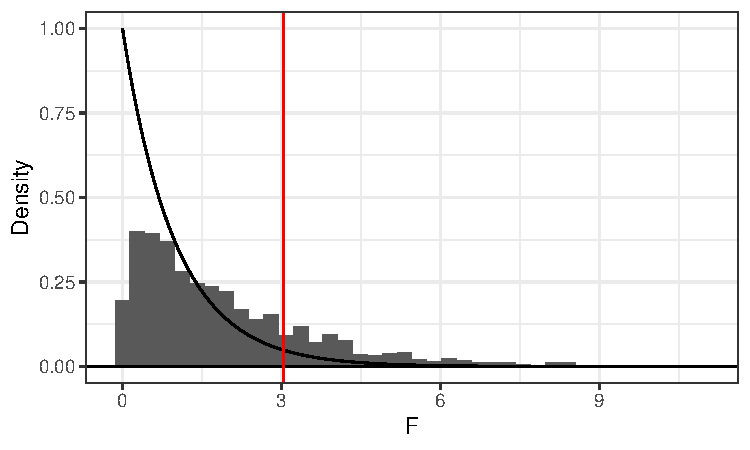
\includegraphics[width=\maxwidth]{figure/unnamed-chunk-13-1} 
\end{knitrout}
\caption{Histogram of F values and the F Distribution (Alternative Hypothesis is True)}\label{F.hist.alt}
\end{figure}

\textcolor{red}{The histogram is more heavily weighted towards the right and doesn't fit the F distribution as well. }

\item Plot a histogram of the $H$ statistics and overlay the sampling 
distribution described by mathematical statisticians in (1). Include a 
vertical line denoting the chi-squared statistic where the rejection region 
starts. What do you note about the histogram and the corresponding $\chi^2$ 
distribution?

\begin{figure}[H]

\centering

\begin{knitrout}\scriptsize
\definecolor{shadecolor}{rgb}{0.969, 0.969, 0.969}\color{fgcolor}\begin{kframe}
\begin{alltt}
\hldef{H_dist} \hlkwb{<-} \hlkwd{tibble}\hldef{(}\hlkwc{H.stat} \hldef{=} \hlkwd{seq}\hldef{(}\hlkwc{from} \hldef{=} \hlnum{0}\hldef{,}
                              \hlkwc{to} \hldef{=} \hlnum{12}\hldef{,}
                              \hlkwc{length.out} \hldef{=} \hlnum{10000}\hldef{)) |>}
  \hlkwd{mutate}\hldef{(}\hlkwc{density} \hldef{=} \hlkwd{dchisq}\hldef{(H.stat,} \hlkwc{df} \hldef{= k}\hlopt{-}\hlnum{1}\hldef{))}

\hldef{rejection_point_H} \hlkwb{<-} \hlkwd{qchisq}\hldef{(}\hlkwc{p} \hldef{=} \hlnum{0.05}\hldef{,} \hlkwc{df} \hldef{= k}\hlopt{-}\hlnum{1}\hldef{,} \hlkwc{lower.tail} \hldef{= F)}


\hlkwd{ggplot}\hldef{()} \hlopt{+}
  \hlkwd{geom_histogram}\hldef{(}\hlkwc{data} \hldef{=} \hlkwd{tibble}\hldef{(}\hlkwc{x} \hldef{= H.stat),} \hlkwd{aes}\hldef{(}\hlkwc{x} \hldef{= x,} \hlkwc{y} \hldef{=} \hlkwd{after_stat}\hldef{(density)),} \hlkwc{bins} \hldef{=} \hlnum{40}\hldef{)} \hlopt{+}
  \hlkwd{geom_line}\hldef{(}\hlkwc{data} \hldef{= H_dist,} \hlkwd{aes}\hldef{(}\hlkwc{x} \hldef{= H.stat,} \hlkwc{y} \hldef{= density))} \hlopt{+}
  \hlkwd{theme_bw}\hldef{()} \hlopt{+}
  \hlkwd{geom_hline}\hldef{(}\hlkwc{yintercept} \hldef{=} \hlnum{0}\hldef{)} \hlopt{+}
  \hlkwd{xlab}\hldef{(}\hlkwd{bquote}\hldef{(chi}\hlopt{^}\hlnum{2}\hldef{))} \hlopt{+}
  \hlkwd{ylab}\hldef{(}\hlsng{"Density"}\hldef{)} \hlopt{+}
  \hlkwd{geom_vline}\hldef{(}\hlkwc{xintercept} \hldef{= rejection_point_H,} \hlkwc{color} \hldef{=} \hlsng{"red"}\hldef{)}
\end{alltt}
\end{kframe}
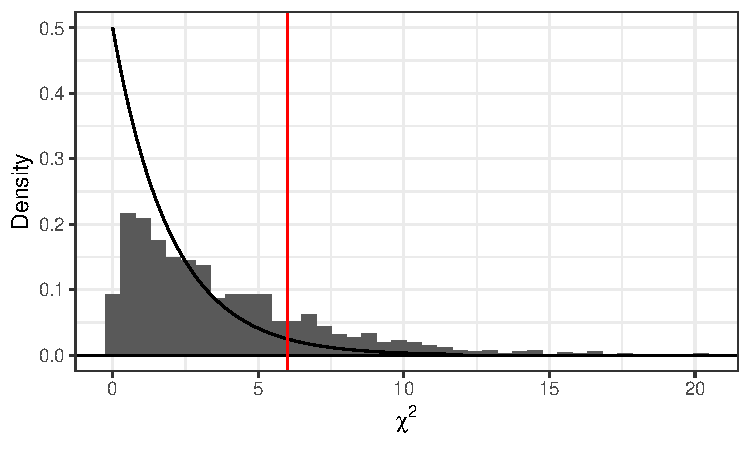
\includegraphics[width=\maxwidth]{figure/unnamed-chunk-14-1} 
\end{knitrout}
\caption{Histogram of H values and the $\chi^2$ Distribution (Alternative is True)}\label{chi2.hist.alt}
\end{figure}

\textcolor{red}{A similar thing happens here as well, where the histogram is weighted to the right a lot more and it doesn't fit the $\chi^2$ distribution as well.}

\item What proportion of the time did your simulation result in a statistic
in the rejection region for both tests?

\begin{knitrout}\scriptsize
\definecolor{shadecolor}{rgb}{0.969, 0.969, 0.969}\color{fgcolor}\begin{kframe}
\begin{alltt}
\hldef{(power_F} \hlkwb{<-} \hlkwd{mean}\hldef{(F.stat} \hlopt{>=} \hldef{rejection_point_F))}
\end{alltt}
\begin{verbatim}
## [1] 0.2
\end{verbatim}
\begin{alltt}
\hldef{(type2_F} \hlkwb{<-} \hlnum{1} \hlopt{-} \hldef{power_F)}
\end{alltt}
\begin{verbatim}
## [1] 0.8
\end{verbatim}
\begin{alltt}
\hldef{(power_H} \hlkwb{<-} \hlkwd{mean}\hldef{(H.stat} \hlopt{>=} \hldef{rejection_point_H))}
\end{alltt}
\begin{verbatim}
## [1] 0.2
\end{verbatim}
\begin{alltt}
\hldef{(type2_H} \hlkwb{<-} \hlnum{1} \hlopt{-} \hldef{power_H)}
\end{alltt}
\begin{verbatim}
## [1] 0.8
\end{verbatim}
\end{kframe}
\end{knitrout}

\item Now, let's assume our data are a bit misbehaved. That is, redo
(a)-(c) but now generate the data from a Laplace distribution with
\texttt{location} equal to $\mu_i$ and the \texttt{scale}=$\sigma_i/\sqrt{2}$.
What do you notice?\\
\textbf{Note:} You can find \texttt{rlaplace()} in the \texttt{VGAM}
package for \texttt{R} \cite{VGAM}.

\begin{knitrout}\scriptsize
\definecolor{shadecolor}{rgb}{0.969, 0.969, 0.969}\color{fgcolor}\begin{kframe}
\begin{alltt}
\hlkwd{library}\hldef{(VGAM)}

\hldef{F.stat_lap} \hlkwb{<-} \hlkwd{rep}\hldef{(}\hlnum{NA}\hldef{,} \hlnum{1000}\hldef{)}
\hldef{H.stat_lap} \hlkwb{<-} \hlkwd{rep}\hldef{(}\hlnum{NA}\hldef{,} \hlnum{1000}\hldef{)}

\hlkwa{for} \hldef{(i} \hlkwa{in} \hlnum{1}\hlopt{:}\hlnum{1000}\hldef{)\{}

\hldef{x1_lap} \hlkwb{<-} \hlkwd{rlaplace}\hldef{(}\hlkwc{n} \hldef{= n1,}
                   \hlkwc{location} \hldef{= mu1,}
                   \hlkwc{scale} \hldef{= sigma}\hlopt{/}\hlkwd{sqrt}\hldef{(}\hlnum{2}\hldef{))}
\hldef{x2_lap} \hlkwb{<-} \hlkwd{rlaplace}\hldef{(}\hlkwc{n} \hldef{= n2,}
                   \hlkwc{location} \hldef{= mu2,}
                   \hlkwc{scale} \hldef{= sigma}\hlopt{/}\hlkwd{sqrt}\hldef{(}\hlnum{2}\hldef{))}
\hldef{x3_lap} \hlkwb{<-} \hlkwd{rlaplace}\hldef{(}\hlkwc{n} \hldef{= n3,}
                   \hlkwc{location} \hldef{= mu3,}
                   \hlkwc{scale} \hldef{= sigma}\hlopt{/}\hlkwd{sqrt}\hldef{(}\hlnum{2}\hldef{))}

  \hlcom{# ANOVA F stat}
  \hldef{xbar1_lap} \hlkwb{<-} \hlkwd{mean}\hldef{(x1_lap)}
  \hldef{xbar2_lap} \hlkwb{<-} \hlkwd{mean}\hldef{(x2_lap)}
  \hldef{xbar3_lap} \hlkwb{<-} \hlkwd{mean}\hldef{(x3_lap)}
  \hldef{X_lap} \hlkwb{<-} \hlkwd{c}\hldef{(x1_lap, x2_lap, x3_lap)}
  \hldef{xbar_lap} \hlkwb{<-} \hlkwd{mean}\hldef{(X_lap)}
  \hlcom{# SSBetween}
  \hldef{SSB_lap} \hlkwb{<-} \hldef{n1}\hlopt{*}\hldef{(xbar1_lap}\hlopt{-}\hldef{xbar_lap)}\hlopt{^}\hlnum{2} \hlopt{+} \hldef{n2}\hlopt{*}\hldef{(xbar2_lap}\hlopt{-}\hldef{xbar_lap)}\hlopt{^}\hlnum{2} \hlopt{+} \hldef{n3}\hlopt{*}\hldef{(xbar3_lap}\hlopt{-}\hldef{xbar_lap)}\hlopt{^}\hlnum{2}
  \hlcom{# SSWithin}
  \hldef{SSW_lap} \hlkwb{<-} \hldef{(n1}\hlopt{-}\hlnum{1}\hldef{)}\hlopt{*}\hlkwd{var}\hldef{(x1_lap)} \hlopt{+} \hldef{(n2}\hlopt{-}\hlnum{1}\hldef{)}\hlopt{*}\hlkwd{var}\hldef{(x2_lap)} \hlopt{+} \hldef{(n3}\hlopt{-}\hlnum{1}\hldef{)}\hlopt{*}\hlkwd{var}\hldef{(x3_lap)}
  \hlcom{# F-statistic}
  \hldef{F.stat_lap[i]} \hlkwb{<-} \hldef{(SSB_lap}\hlopt{/}\hldef{(k}\hlopt{-}\hlnum{1}\hldef{))}\hlopt{/}\hldef{(SSW_lap}\hlopt{/}\hldef{(N}\hlopt{-}\hldef{k))}

  \hlcom{# KW H stat}
  \hldef{X_lap} \hlkwb{<-} \hlkwd{c}\hldef{(x1_lap, x2_lap, x3_lap)}
  \hldef{ranks_lap} \hlkwb{<-} \hlkwd{rank}\hldef{(X_lap)}
  \hldef{r1_lap} \hlkwb{<-} \hldef{ranks_lap[}\hlnum{1}\hlopt{:}\hlkwd{length}\hldef{(x1_lap)]}
  \hldef{r2_lap} \hlkwb{<-} \hldef{ranks_lap[(n1}\hlopt{+}\hlnum{1}\hldef{)}\hlopt{:}\hldef{(n1}\hlopt{+}\hldef{n2)]}
  \hldef{r3_lap} \hlkwb{<-} \hldef{ranks_lap[(n1}\hlopt{+}\hldef{n2}\hlopt{+}\hlnum{1}\hldef{)}\hlopt{:}\hldef{N]}
  \hlcom{# Rank Sums}
  \hldef{rank.sums_lap} \hlkwb{<-} \hlnum{12}\hlopt{/}\hldef{(N}\hlopt{*}\hldef{(N}\hlopt{+}\hlnum{1}\hldef{))} \hlopt{*} \hldef{(}\hlkwd{sum}\hldef{(r1_lap)}\hlopt{^}\hlnum{2}\hlopt{/}\hldef{n1} \hlopt{+} \hlkwd{sum}\hldef{(r2_lap)}\hlopt{^}\hlnum{2}\hlopt{/}\hldef{n2} \hlopt{+} \hlkwd{sum}\hldef{(r3_lap)}\hlopt{^}\hlnum{2}\hlopt{/}\hldef{n3)}
  \hlcom{# Ties? (Note: when there are no ties, this adjustment is 1)}
  \hldef{ties.adj_lap} \hlkwb{<-} \hlkwd{tibble}\hldef{(}\hlkwc{r}\hldef{=ranks_lap) |>} \hlcom{# create a tibble}
    \hlkwd{group_by}\hldef{(r) |>}               \hlcom{# group by the ranks}
    \hlkwd{summarize}\hldef{(}\hlkwc{n}\hldef{=}\hlkwd{n}\hldef{())|>}           \hlcom{# count the number of unique ranks}
    \hlkwd{summarize}\hldef{(}\hlkwc{ties.adj} \hldef{=} \hlnum{1}\hlopt{-}\hlkwd{sum}\hldef{(n}\hlopt{^}\hlnum{3}\hlopt{-}\hldef{n)}\hlopt{/}\hldef{(N}\hlopt{^}\hlnum{3}\hlopt{-}\hldef{N))|>} \hlcom{# compute adjustment}
    \hlkwd{pull}\hldef{()} \hlcom{# convert from tibble to numeric}
  \hlcom{# H-statistic}
  \hldef{H.stat_lap[i]} \hlkwb{<-} \hldef{(rank.sums_lap} \hlopt{-} \hlnum{3}\hlopt{*}\hldef{(N}\hlopt{+}\hlnum{1}\hldef{))}\hlopt{/}\hldef{ties.adj_lap}

\hldef{\}}
\end{alltt}
\end{kframe}
\end{knitrout}

\begin{figure}[H]

\centering

\begin{knitrout}\scriptsize
\definecolor{shadecolor}{rgb}{0.969, 0.969, 0.969}\color{fgcolor}\begin{kframe}
\begin{alltt}
\hlkwd{ggplot}\hldef{()} \hlopt{+}
  \hlkwd{geom_histogram}\hldef{(}\hlkwc{data} \hldef{=} \hlkwd{tibble}\hldef{(}\hlkwc{x} \hldef{= F.stat_lap),} \hlkwd{aes}\hldef{(}\hlkwc{x} \hldef{= x,} \hlkwc{y} \hldef{=} \hlkwd{after_stat}\hldef{(density)),} \hlkwc{bins} \hldef{=} \hlnum{40}\hldef{)} \hlopt{+}
  \hlkwd{geom_line}\hldef{(}\hlkwc{data} \hldef{= F_dist,} \hlkwd{aes}\hldef{(}\hlkwc{x} \hldef{= F.stat,} \hlkwc{y} \hldef{= density))} \hlopt{+}
  \hlkwd{theme_bw}\hldef{()} \hlopt{+}
  \hlkwd{geom_hline}\hldef{(}\hlkwc{yintercept} \hldef{=} \hlnum{0}\hldef{)} \hlopt{+}
  \hlkwd{xlab}\hldef{(}\hlsng{"F"}\hldef{)} \hlopt{+}
  \hlkwd{ylab}\hldef{(}\hlsng{"Density"}\hldef{)} \hlopt{+}
  \hlkwd{geom_vline}\hldef{(}\hlkwc{xintercept} \hldef{= rejection_point_F,} \hlkwc{color} \hldef{=} \hlsng{"red"}\hldef{)}
\end{alltt}
\end{kframe}
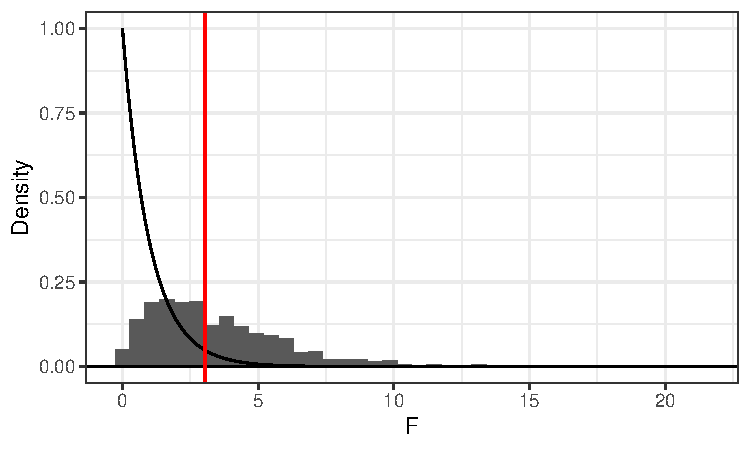
\includegraphics[width=\maxwidth]{figure/unnamed-chunk-17-1} 
\end{knitrout}
\caption{Histogram of F values and the F Distribution (Data is Laplace Distributed and Alternative is True)}\label{F.hist.lap.alt}
\end{figure}

\begin{figure}[H]

\centering

\begin{knitrout}\scriptsize
\definecolor{shadecolor}{rgb}{0.969, 0.969, 0.969}\color{fgcolor}\begin{kframe}
\begin{alltt}
\hlkwd{ggplot}\hldef{()} \hlopt{+}
  \hlkwd{geom_histogram}\hldef{(}\hlkwc{data} \hldef{=} \hlkwd{tibble}\hldef{(}\hlkwc{x} \hldef{= H.stat_lap),} \hlkwd{aes}\hldef{(}\hlkwc{x} \hldef{= x,} \hlkwc{y} \hldef{=} \hlkwd{after_stat}\hldef{(density)),} \hlkwc{bins} \hldef{=} \hlnum{40}\hldef{)} \hlopt{+}
  \hlkwd{geom_line}\hldef{(}\hlkwc{data} \hldef{= H_dist,} \hlkwd{aes}\hldef{(}\hlkwc{x} \hldef{= H.stat,} \hlkwc{y} \hldef{= density))} \hlopt{+}
  \hlkwd{theme_bw}\hldef{()} \hlopt{+}
  \hlkwd{geom_hline}\hldef{(}\hlkwc{yintercept} \hldef{=} \hlnum{0}\hldef{)} \hlopt{+}
  \hlkwd{xlab}\hldef{(}\hlkwd{bquote}\hldef{(chi}\hlopt{^}\hlnum{2}\hldef{))} \hlopt{+}
  \hlkwd{ylab}\hldef{(}\hlsng{"Density"}\hldef{)} \hlopt{+}
  \hlkwd{geom_vline}\hldef{(}\hlkwc{xintercept} \hldef{= rejection_point_H,} \hlkwc{color} \hldef{=} \hlsng{"red"}\hldef{)}
\end{alltt}
\end{kframe}
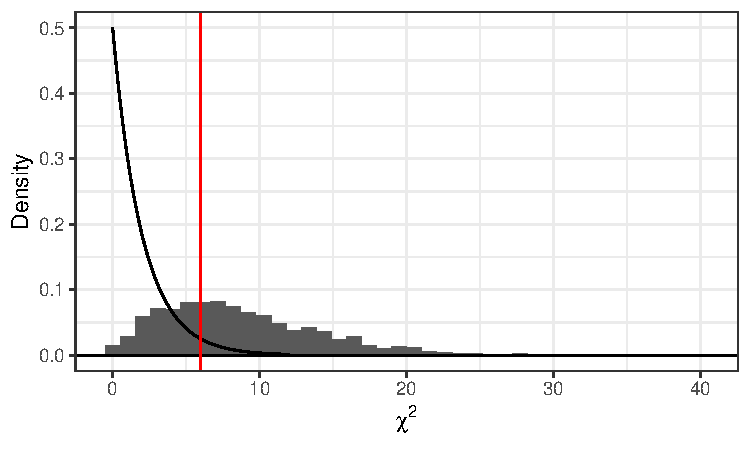
\includegraphics[width=\maxwidth]{figure/unnamed-chunk-18-1} 
\end{knitrout}
\caption{Histogram of H values and the $\chi^2$ Distribution (Data is Laplace Distributed and Alternative is True)}\label{H.hist.lap.alt}
\end{figure}


\begin{knitrout}\scriptsize
\definecolor{shadecolor}{rgb}{0.969, 0.969, 0.969}\color{fgcolor}\begin{kframe}
\begin{alltt}
\hldef{(power_F_lap} \hlkwb{<-} \hlkwd{mean}\hldef{(F.stat_lap} \hlopt{>=} \hldef{rejection_point_F))}
\end{alltt}
\begin{verbatim}
## [1] 0.469
\end{verbatim}
\begin{alltt}
\hldef{(type2_F_lap} \hlkwb{<-} \hlnum{1} \hlopt{-} \hldef{power_F_lap)}
\end{alltt}
\begin{verbatim}
## [1] 0.531
\end{verbatim}
\begin{alltt}
\hldef{(power_H_lap} \hlkwb{<-} \hlkwd{mean}\hldef{(H.stat_lap} \hlopt{>=} \hldef{rejection_point_H))}
\end{alltt}
\begin{verbatim}
## [1] 0.64
\end{verbatim}
\begin{alltt}
\hldef{(type2_H_lap} \hlkwb{<-} \hlnum{1} \hlopt{-} \hldef{power_H_lap)}
\end{alltt}
\begin{verbatim}
## [1] 0.36
\end{verbatim}
\end{kframe}
\end{knitrout}

\textcolor{red}{The power increases when the data is Laplace distributed. This makes sense as the Kruskal-Wallis test doesn't assume normality within each group.}


\end{enumerate} 
%%%%%%%%%%%%%%%%%%%%%%%%%%%%%%%%%%%%%%%%%%%%%%%%%%%%%%%%%%%%%%%%%%%%%%%%%%%%%%%%
%%%%%%%%%%%%%%%%%%%%%%%%%%%%%%%%%%%%%%%%%%%%%%%%%%%%%%%%%%%%%%%%%%%%%%%%%%%%%%%%
% Question 3
%%%%%%%%%%%%%%%%%%%%%%%%%%%%%%%%%%%%%%%%%%%%%%%%%%%%%%%%%%%%%%%%%%%%%%%%%%%%%%%%
%%%%%%%%%%%%%%%%%%%%%%%%%%%%%%%%%%%%%%%%%%%%%%%%%%%%%%%%%%%%%%%%%%%%%%%%%%%%%%%%
\item \textbf{What does it mean?} Take a moment to reflect on (1) and (2).
\begin{enumerate}
\item What is the estimated Type I error, Type II error, and Power for the
scenarios you simulated in (1) and (2) when the data are drawn from Gaussian 
distributions? When the data are drawn from Laplace distributions? Why
do you think you are seeing the relationship(s) you see?

\begin{knitrout}\scriptsize
\definecolor{shadecolor}{rgb}{0.969, 0.969, 0.969}\color{fgcolor}\begin{kframe}
\begin{alltt}
\hlkwd{library}\hldef{(xtable)}

\hldef{normal_table} \hlkwb{<-} \hlkwd{tibble}\hldef{(}\hlkwc{Method} \hldef{=} \hlkwd{c}\hldef{(}\hlsng{"ANOVA"}\hldef{,} \hlsng{"Kruskal Wallis"}\hldef{),}
                       \hlkwc{`Type I Error`} \hldef{=} \hlkwd{c}\hldef{(type1_error_F, type1_error_H),}
                       \hlkwc{`Type II Error`}\hldef{=} \hlkwd{c}\hldef{(type2_F, type2_H),}
                       \hlkwc{`Power`} \hldef{=} \hlkwd{c}\hldef{(power_F, power_H))}
\hldef{normal_table} \hlkwb{<-} \hlkwd{xtable}\hldef{(normal_table,}\hlkwc{label} \hldef{=} \hlsng{"normal.tab"}\hldef{,} \hlkwc{caption} \hldef{=} \hlsng{"Normally Distributed Data"}\hldef{)}

\hldef{laplace_table} \hlkwb{<-} \hlkwd{tibble}\hldef{(}\hlkwc{Method} \hldef{=} \hlkwd{c}\hldef{(}\hlsng{"ANOVA"}\hldef{,} \hlsng{"Kruskal Wallis"}\hldef{),}
                        \hlkwc{`Type I Error`} \hldef{=} \hlkwd{c}\hldef{(type1_error_F_lap, type1_error_H_lap),}
                       \hlkwc{`Type II Error`}\hldef{=} \hlkwd{c}\hldef{(type2_F_lap, type2_H_lap),}
                       \hlkwc{`Power`} \hldef{=} \hlkwd{c}\hldef{(power_F_lap, power_H_lap))}
\hldef{laplace_table} \hlkwb{<-} \hlkwd{xtable}\hldef{(laplace_table,}\hlkwc{label} \hldef{=} \hlsng{"laplace.tab"}\hldef{,} \hlkwc{caption} \hldef{=} \hlsng{"Laplace Distributed Data"}\hldef{)}
\end{alltt}
\end{kframe}
\end{knitrout}


% latex table generated in R 4.5.1 by xtable 1.8-4 package
% Sun Oct 19 16:38:43 2025
\begin{table}[H]
\centering
\begingroup\small
\begin{tabular}{lrrr}
  \hline
Method & Type I Error & Type II Error & Power \\ 
  \hline
ANOVA & 0.05 & 0.80 & 0.20 \\ 
  Kruskal Wallis & 0.05 & 0.80 & 0.20 \\ 
   \hline
\end{tabular}
\endgroup
\caption{Normally Distributed Data} 
\label{normal.tab}
\end{table}



% latex table generated in R 4.5.1 by xtable 1.8-4 package
% Sun Oct 19 16:38:43 2025
\begin{table}[H]
\centering
\begingroup\small
\begin{tabular}{lrrr}
  \hline
Method & Type I Error & Type II Error & Power \\ 
  \hline
ANOVA & 0.05 & 0.53 & 0.47 \\ 
  Kruskal Wallis & 0.05 & 0.36 & 0.64 \\ 
   \hline
\end{tabular}
\endgroup
\caption{Laplace Distributed Data} 
\label{laplace.tab}
\end{table}


\textcolor{red}{In the gaussian data, we see that when our data match our assumptions of the distributions, the results of each test are exactly the same. We might usually expect to see a slightly higher power in the ANOVA test compared to the non-parametric alternative, although here that is not the case.}

\textcolor{red}{In the Laplace distributed data, we see that when our data doesn't match our assumptions of the distributions, the results of each test are different. The non-parametric alternative that doesn't assume normality is more powerful than the standard test that does.}

\item When we find a statistically discernible result, this means that we 
have found support for the alternative, or something unusual has occurred. 
Tie this statement to your results in (1) and (2).

\textcolor{red}{When we find a statistically discernible result, we have indications that our assumptions about the data are incorrect. The more assumptions are incorrect, the more evidence that we're going to have in the alternative. That's why we see that when the means are not the same, and the distributions are not normal, we have a higher power than when just the means are different.}

\item When we find a non-statistically discernible result, this means that
we have not found support for the alternative, or we did not find 
\emph{enough} support for the alternative. Tie this statement to your 
results in (1) and (2).

\textcolor{red}{As we can see from the tables, the rate of a type I error remains constant across means and distributions. This shows us that our cautiousness over incorrectly rejecting the null stays consistent and is robust across conditions like distribution.}

\item In as few words as possible, describe a hypothesis test. Your solution
must include reference(s) to a statistic and a sampling distribution either 
directly or indirectly.

\textcolor{red}{We're testing how weird a statistic calculated of of our data is given an assumed random distribution of that statistic.}

\end{enumerate}
%%%%%%%%%%%%%%%%%%%%%%%%%%%%%%%%%%%%%%%%%%%%%%%%%%%%%%%%%%%%%%%%%%%%%%%%%%%%%%%%
%%%%%%%%%%%%%%%%%%%%%%%%%%%%%%%%%%%%%%%%%%%%%%%%%%%%%%%%%%%%%%%%%%%%%%%%%%%%%%%%
% Question 4
%%%%%%%%%%%%%%%%%%%%%%%%%%%%%%%%%%%%%%%%%%%%%%%%%%%%%%%%%%%%%%%%%%%%%%%%%%%%%%%%
%%%%%%%%%%%%%%%%%%%%%%%%%%%%%%%%%%%%%%%%%%%%%%%%%%%%%%%%%%%%%%%%%%%%%%%%%%%%%%%%
\item \textbf{What do we do IRL?} \cite{Wang24} investigated how different
types of plastic pollution (microplastics) contribute to antibiotic resistance.\\

The researchers collected soil from the Ecological Research Station for 
Grassland Farming in the Jilin Province of Northeast China. They filled
circular plastic pots with a mixture of the collected soil, gravel, and 24 mL 
of microplastics, varying the number of types -- one, three, and six from
twelve microplastics commonly found in soil environments. In each pot, they 
planted one or multiple species and either applied a fungicide treatment
or the equivalent amount of water.\\

One outcome of interest is how the microplastic diversity, fungicide 
application, or number of species per pot impacts the number of copies
of antibiotic resistance genes (ARGs) per cell.\\

I have loaded the data below:
\begin{knitrout}\scriptsize
\definecolor{shadecolor}{rgb}{0.969, 0.969, 0.969}\color{fgcolor}\begin{kframe}
\begin{alltt}
\hldef{dat} \hlkwb{<-} \hlkwd{read_csv}\hldef{(}\hlsng{"Wang2025.csv"}\hldef{)}

\hldef{long_dat} \hlkwb{<-} \hldef{dat |>}
  \hlkwd{pivot_longer}\hldef{(}\hlkwc{cols} \hldef{=} \hlkwd{c}\hldef{(}\hlsng{"MP diversity"}\hldef{,} \hlsng{"Fungicide application"}\hldef{,} \hlsng{"Plant community"}\hldef{),}
               \hlkwc{names_to} \hldef{=} \hlsng{"Comparison"}\hldef{,}
               \hlkwc{values_to} \hldef{=} \hlsng{"Group"}\hldef{)}

\hldef{summary_dat} \hlkwb{<-} \hldef{long_dat |>}
  \hlkwd{group_by}\hldef{(Comparison, Group) |>}
  \hlkwd{summarise}\hldef{(}\hlkwc{mean} \hldef{=} \hlkwd{mean}\hldef{(`Copies of ARGs per cell`),}
            \hlkwc{SEM} \hldef{=} \hlkwd{sd}\hldef{(`Copies of ARGs per cell`)} \hlopt{/} \hlkwd{sqrt}\hldef{(}\hlkwd{n}\hldef{()))}
\end{alltt}
\end{kframe}
\end{knitrout}
\begin{enumerate}
\item Summarize the data. Note that the authors do an okay job of graphing the
data in Figure 1b.

\begin{figure}[H]

\centering

\begin{knitrout}\scriptsize
\definecolor{shadecolor}{rgb}{0.969, 0.969, 0.969}\color{fgcolor}\begin{kframe}
\begin{alltt}
\hlkwd{ggplot}\hldef{(}\hlkwc{data} \hldef{= summary_dat,} \hlkwd{aes}\hldef{(}\hlkwc{x} \hldef{= Group,} \hlkwc{y} \hldef{= mean,} \hlkwc{fill} \hldef{= Group))} \hlopt{+}
  \hlkwd{geom_col}\hldef{()} \hlopt{+}
  \hlkwd{facet_wrap}\hldef{(}\hlsng{"Comparison"}\hldef{,} \hlkwc{scales} \hldef{=} \hlsng{"free_x"}\hldef{)} \hlopt{+}
  \hlkwd{geom_errorbar}\hldef{(}\hlkwd{aes}\hldef{(}\hlkwc{ymin} \hldef{= mean} \hlopt{-} \hlnum{2}\hlopt{*}\hldef{SEM,} \hlkwc{ymax} \hldef{= mean} \hlopt{+} \hlnum{2}\hlopt{*}\hldef{SEM),} \hlkwc{width} \hldef{=} \hlnum{0.25}\hldef{)} \hlopt{+}
  \hlkwd{geom_hline}\hldef{(}\hlkwc{yintercept} \hldef{=} \hlnum{0}\hldef{)} \hlopt{+}
  \hlkwd{scale_fill_grey}\hldef{()} \hlopt{+}
  \hlkwd{theme_bw}\hldef{()} \hlopt{+}
  \hlkwd{xlab}\hldef{(}\hlsng{''}\hldef{)} \hlopt{+}
  \hlkwd{ylab}\hldef{(}\hlsng{'Mean ARGs/cell +/- 2 * SEM'}\hldef{)} \hlopt{+}
  \hlkwd{guides}\hldef{(}\hlkwc{fill} \hldef{=} \hlsng{"none"}\hldef{)}
\end{alltt}
\end{kframe}
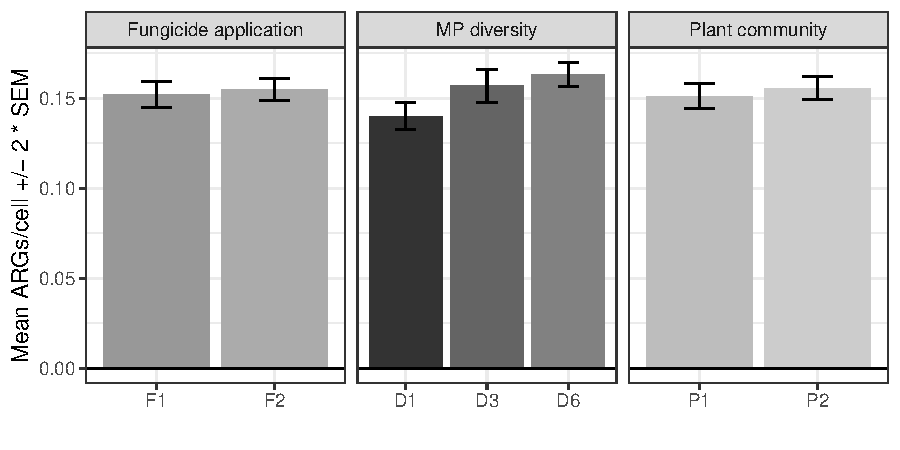
\includegraphics[width=\maxwidth]{figure/unnamed-chunk-24-1} 
\end{knitrout}

\label{plastic.sum}
\caption{ARGs/Cell Across a) Fungicide Application, b) Microplastic Diversity, and c) Plant Community}
\end{figure}


\item The authors perform a Kruskal-Wallis test. Is that necessary? Is it
appropriate? 

\begin{figure}[H]

\centering

\begin{knitrout}\scriptsize
\definecolor{shadecolor}{rgb}{0.969, 0.969, 0.969}\color{fgcolor}
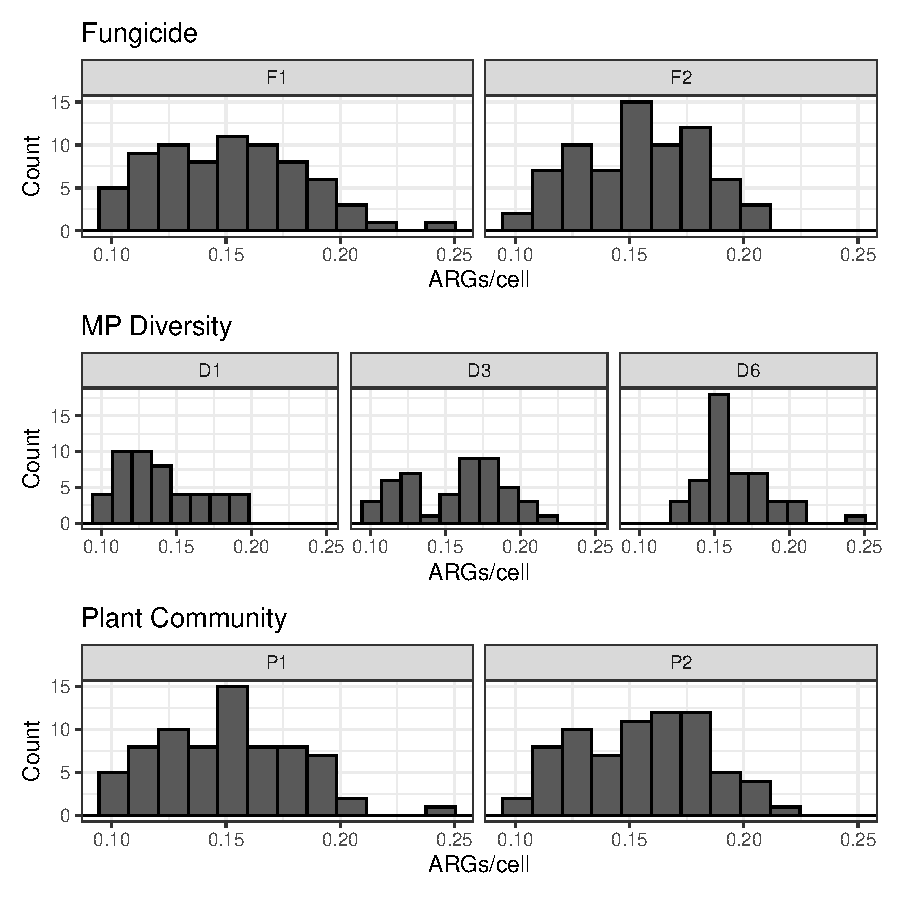
\includegraphics[width=\maxwidth]{figure/unnamed-chunk-25-1} 
\end{knitrout}

\label{plastic.hists}
\caption{Histogram of Comparison Groups}
\end{figure}

\textcolor{red}{(Sorry, I couldn't fit all the code with the plot)}

\textcolor{red}{Looking at the histograms of all the groups, all of the groups appear approximately normal. Therefore, Using an ANOVA or Welch's ANOVA seems appropriate for this data.}

\item Perform the Kruskal-Wallis test to assess whether the number of copies
of antibiotic resistance genes (ARGs) per cell differs across microplastic 
diversity. Note that you can compute the effect size using
\[\eta^2 = \frac{H-k+1}{N-k},\]
which indicates effect sizes of minuscule ($<0.01$), small ($0.01-0.06$), 
moderate ($0.06-0.14$) and large ($\geq 0.14$).\\

\begin{knitrout}\scriptsize
\definecolor{shadecolor}{rgb}{0.969, 0.969, 0.969}\color{fgcolor}\begin{kframe}
\begin{alltt}
\hlkwd{library}\hldef{(stats)}

\hldef{k} \hlkwb{=} \hlnum{3}
\hldef{N} \hlkwb{=} \hlnum{144}

\hldef{(test} \hlkwb{<-} \hlkwd{kruskal.test}\hldef{(`Copies of ARGs per cell`} \hlopt{~} \hldef{Group,} \hlkwc{data} \hldef{= mp_diversity))}
\end{alltt}
\begin{verbatim}
## 
## 	Kruskal-Wallis rank sum test
## 
## data:  Copies of ARGs per cell by Group
## Kruskal-Wallis chi-squared = 16.325, df = 2, p-value = 0.0002851
\end{verbatim}
\begin{alltt}
\hldef{(eta2} \hlkwb{<-} \hldef{(}\hlkwd{unname}\hldef{(test}\hlopt{$}\hldef{statistic)} \hlopt{-} \hldef{k} \hlopt{+} \hlnum{1}\hldef{)} \hlopt{/} \hldef{(N} \hlopt{-} \hldef{k))}
\end{alltt}
\begin{verbatim}
## [1] 0.1015978
\end{verbatim}
\end{kframe}
\end{knitrout}

\textcolor{red}{After performing a Kruskal-Wallis test, we obtain a test statistic $\chi^2$ of 16.325 ($p = 0.0003$, $\eta^2 = 0.10$). This tells us that there is a statistcally discernible difference in ARGs across types of microplastic diversity because $p < \alpha = 0.05$. A $\eta^2$ of 0.10 tells us that the effect of microplastic diversity on ARGs is moderate.}

\item If the test in the previous part is statistically discernible, conduct
Dunn's post hoc procedure, which evaluates whether it is equally likely that a 
random observation from sample $i$ is	larger than a random observation from 
sample $j$,
\begin{align*}
H_0&: P(X_i>X_j)=0.50\\
H_a&: P(X_i>X_j) \neq 0.50.
\end{align*}
The \textbf{test statistic} for this test is 
\[z_{ij} = \frac{\bar{R}_{i\cdot} - \bar{R}_{j\cdot}}{\sqrt{\left[\frac{N(N+1)}{12} - \frac{\sum_{r=1}^{\max(r)} o_r^3-o_r}{12(N-1)}\right]\left(\frac{1}{n_i}+\frac{1}{n_j}\right)}} \sim \mathcal{AG}(\mu_z=0,\sigma_z=1),\]
where $\bar{R}_{i\cdot}$ and $\bar{R}_{j\cdot}$ are the mean of the ranks for sample $i$ and sample $j$, and $o_r$ is the number of times rank $r$ occurs.\\

An \textbf{effect size} can be computed similarly to the two-sample signed-rank test:
\[r = \frac{z_{ij}}{\sqrt{n_i+n_j}},\]
which can be interpreted as minuscule ($<0.10$), small ($0.10-0.30$), 
moderate ($0.30-0.50$) or large ($\geq 0.50$).

The $p$-value for the test of difference between group $i$ and $j$ is $2P(Z<-|z_{ij}|).$\\

\textbf{Hint:} This analyses can be conducted using \texttt{dunn\_test()} from
the \texttt{rstatix} package \cite{rstatix}.

\begin{knitrout}\scriptsize
\definecolor{shadecolor}{rgb}{0.969, 0.969, 0.969}\color{fgcolor}\begin{kframe}
\begin{alltt}
\hlkwd{library}\hldef{(rstatix)}

\hldef{posthoc_sum} \hlkwb{<-} \hlkwd{dunn_test}\hldef{(}\hlkwc{data} \hldef{= mp_diversity, `Copies of ARGs per cell`} \hlopt{~} \hldef{Group) |>}
  \hlkwd{mutate}\hldef{(}\hlkwc{`Effect Size`} \hldef{= statistic} \hlopt{/} \hldef{(}\hlkwd{sqrt}\hldef{(n1}\hlopt{+}\hldef{n2))) |>}
  \hlkwd{select}\hldef{(}\hlopt{-}\hldef{.y.,}
         \hlopt{-}\hldef{n1,}
         \hlopt{-}\hldef{n2) |>}
  \hlkwd{rename}\hldef{(}\hlsng{"Group 1"} \hldef{= group1,}
         \hlsng{"Group 2"} \hldef{= group2,}
         \hlkwc{Z} \hldef{= statistic,}
         \hlkwc{Adjusted} \hldef{= p.adj,}
         \hlsng{"Significance"} \hldef{= p.adj.signif) |>}
  \hlkwd{mutate}\hldef{(}\hlkwc{p} \hldef{=} \hlkwd{ifelse}\hldef{(p} \hlopt{<} \hlnum{0.001}\hldef{,} \hlsng{"<0.001"}\hldef{,} \hlkwd{round}\hldef{(p,} \hlnum{3}\hldef{)) ,}
         \hlkwc{Interpretation} \hldef{=} \hlkwd{case_when}\hldef{(`Effect Size`} \hlopt{<} \hlnum{0.1} \hlopt{~} \hlsng{"miniscule"}\hldef{,}
                                    \hldef{`Effect Size`} \hlopt{>=} \hlnum{0.1} \hlopt{&} \hldef{`Effect Size`} \hlopt{<} \hlnum{0.3} \hlopt{~} \hlsng{"small"}\hldef{,}
                                    \hldef{`Effect Size`} \hlopt{>=} \hlnum{0.3} \hlopt{&} \hldef{`Effect Size`} \hlopt{<} \hlnum{0.5} \hlopt{~} \hlsng{"moderate"}\hldef{,}
                                    \hldef{`Effect Size`} \hlopt{>=} \hlnum{0.5} \hlopt{~} \hlsng{"large"}\hldef{),}
         \hlkwc{Adjusted} \hldef{=} \hlkwd{ifelse}\hldef{(Adjusted} \hlopt{<} \hlnum{0.001}\hldef{,} \hlsng{"<0.001"}\hldef{,} \hlkwd{round}\hldef{(Adjusted,} \hlnum{3}\hldef{)))}


\hldef{posthoc_sum} \hlkwb{<-} \hlkwd{xtable}\hldef{(posthoc_sum,}\hlkwc{label} \hldef{=} \hlsng{"posthoc.tab"}\hldef{,} \hlkwc{caption} \hldef{=} \hlsng{"Posthoc Summary"}\hldef{,} \hlkwc{digits} \hldef{=} \hlnum{3}\hldef{)}
\end{alltt}
\end{kframe}
\end{knitrout}


% latex table generated in R 4.5.1 by xtable 1.8-4 package
% Sun Oct 19 16:38:46 2025
\begin{table}[H]
\centering
\begingroup\small
\begin{tabular}{llrlllrl}
  \hline
Group 1 & Group 2 & Z & p & Adjusted & Significance & Effect Size & Interpretation \\ 
  \hline
D1 & D3 & 2.995 & 0.003 & 0.005 & ** & 0.306 & moderate \\ 
  D1 & D6 & 3.846 & $<$0.001 & $<$0.001 & *** & 0.393 & moderate \\ 
  D3 & D6 & 0.851 & 0.395 & 0.395 & ns & 0.087 & miniscule \\ 
   \hline
\end{tabular}
\endgroup
\caption{Posthoc Summary} 
\label{posthoc.tab}
\end{table}


\textcolor{red}{After performing a posthoc Dunn's test, we see that there are statistically discernible differences between groups: D1 vs. D3 ($Z = 2.995$, $p = 0.005$, $r = 0.306$) and D1 vs. D6 ($Z = 3.846$, $p < 0.001$, $r = 0.393$). Combined with the visuals in b) of Figure \ref{plastic.sum} and the effect sizes ($r$), we can say that D3 has moderately more ARGs than D1, and D6 has moderately more ARGs than D3. The difference between D3 and D6 did not reach traditional levels of statistical significance.}



\end{enumerate}
\end{enumerate}
\bibliography{bib}
\end{document}
